% !TEX root = main.tex

\chapter{Background}
\label{ch:background}
\noindent

\red{TODO: fix fig name}


\section{WebAssembly}
\label{sec:webassembly}


% breif overview
WebAssembly~\cite{wasm} is a low-level bytecode language that is safe, fast,
portable, and compact.
It is widely used as a compile target for web applications.
Not only that, other areas such as edge computing~\cite{wasm-edge},
IoT~\cite{wasm-iot}, and block chains~\cite{wasm-block} deploy the advantages
of WebAssembly.


% risk of implementation divergence
There are dozens of WebAssembly engines; all the browsers have there own
implementations of WebAssembly with multiple tiers ~\cite{v8}
\cite{spidermonkey} \cite{webkit}, and there are many engines that target for
specific areas including embedded systems and edge computing.
However, as WebAssembly should be portable across these implementations, it risks
the implementations divergence.


% rigorous standardization -> spec is rigorous: formal notation & prose notation
To mitigate this problem, WebAssembly has been standardized very rigourously by
the W3C~\cite{wasm-w3c}.
Especially, WebAssembly specification document is written very rigorously.
It describes the semantics of WebAssembly in two forms: formal notation and
prose notation.
Formal notation uses mathematical rules to compactly describe the semantics,
and it is used for proofs such as type soundness.
On the other hand, prose notation uses psudocodes algorithm to explain the
semantics through a step by step instruction.
Most WebAssembly users and engine developers are not familiar with
mathematical rules, so they utilize the prose notation.


% structure
A WebAssembly program is comprised of \textit{modules}.
A module is the unit of deployment, loading, and compilation, which consists of
definitions such as functions, globals, and memories.
A module is instantiated to validate the module and allocate each definition to
the data structure named \textit{store}.
This results in a module instance, a runtime representation for the module.
After the instantiation, functions can be invoked so that the function body,
which is a sequence of instructions, is executed.


% execution
WebAssembly execution is based on a stack machine.
An instruction consumes values in the stack as operands, performs some
operation, produces resulting values, and pushes them to the stack.
\cref{fig:testop} is the WebAssembly specification document for the
\texttt{testop} instruction.
Prose notation is written in the upper part, and formal notation is written in
the lower grey box.
In the prose notation, it pops a value from the stack, performs a test
operation, and pushes the result to the stack.
It is written compactly in the form of reduction rule in the formal notation
which consists of LHS, RHS, and premises: $(t.const ~ c_1) ~ t.testop$,
$(i32.const ~ c)$, and $c = testop_t(c_1)$.
The LHS means that the value at the top of the stack is $(t.const ~ c_1)$,
and an instruction to execute is $t.testop$.
The RHS means that the value at the top of the stack is changed to $(i32.const
~ c)$, and this happens when the premise $c = testop_t(c_1)$ is satisfied.


% control structure
The stack stores not only the input and output values of the instructions but also
structures related to the control flow.
A \textit{call frame} and a \textit{label} are used for function call and
branching, respectively.
In exception handling proposal, there is a \textit{handler} for exception
handling, and other strucutres could be introduced in the future.
How these control structures are used for the control flow will be discussed in
\cref{sec:control flow in official prose}.



\newcommand{\officialp}{official prose}
\newcommand{\spectecp}{SpecTec prose}

\red{TODO: explanation of the terms \officialp{} and \spectecp{}} \\
\red{TODO: remove redundant part in the fig} \\
\red{TODO: explanation of context(frame/label): in the background? or here?} \\
\red{TODO: the notion of meta-level interpreter in background} \\
\red{TODO: try finding better terminology rather than "model"} \\

\section{Control flow in official prose}
\label{sec:control flow in official prose}

% control flow structure in official prose
It might be easy to understand how the \officialp{} explains the control flow
of WebAssembly, if we assume that a WebAssembly code is loaded on a memory and
a pc points to the instruction to execute.
To describe control flow, it uses a structure named \textit{block} which
consitutes of a instruction sequence.
When executing the instructions in the block, pc can be changed to the starting
point of the block or the end of the block.


% an example of Wasm control flow in official prose
\begin{example}
\label{ex:br}
\begin{verbatim}
  // infinite loop
  (loop (result i32) (i32.const 42) (br 0) (unreachable) end) (unreachable)
\end{verbatim}
\end{example}

\cref{ex:br} is a WebAssembly code example that has \texttt{loop} and
\texttt{unreachable}
Here, result type of the \texttt{loop} is \texttt{i32} and the \texttt{loop}
has a block of three instructions: \texttt{i32.const}, \texttt{br}, and
\texttt{unreachable}.
\cref{fig:loop} is the \officialp{} of the \texttt{loop} instruction.
It says that the continuation is the start of the loop, the information is
stored in a label, and it \textit{enters} the block with the label.
The term \textit{enter} means that it pushes the label in the stack and makes
pc points to the first instruction in the block.
The \texttt{i32.const} instruction is executed first, which just pushes the
\texttt{i32} value \texttt{42} in the stack.
Then, The \texttt{br} instruction is executed.
\cref{fig:br} is the \officialp{} of the \texttt{br} instruction.
It pops the label from the stack, and makes pc points to the continuation of
the label, which is the start of the loop instruction.
As a result, the code example above is a infinite loop pushing \texttt{42}
forever without executing \texttt{unreachable} instructions.

\begin{figure}[h!]
    \centerline{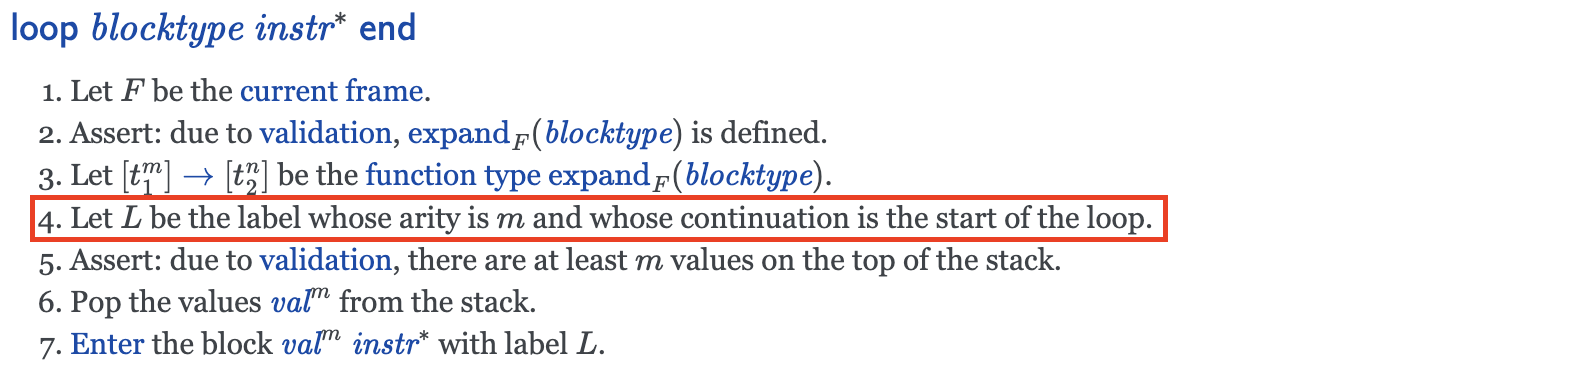
\includegraphics[width=15cm]{fig/loop}}
    \caption[Enter the caption title here]{\texttt{loop} instruction} \label{fig:loop}
    \centerline{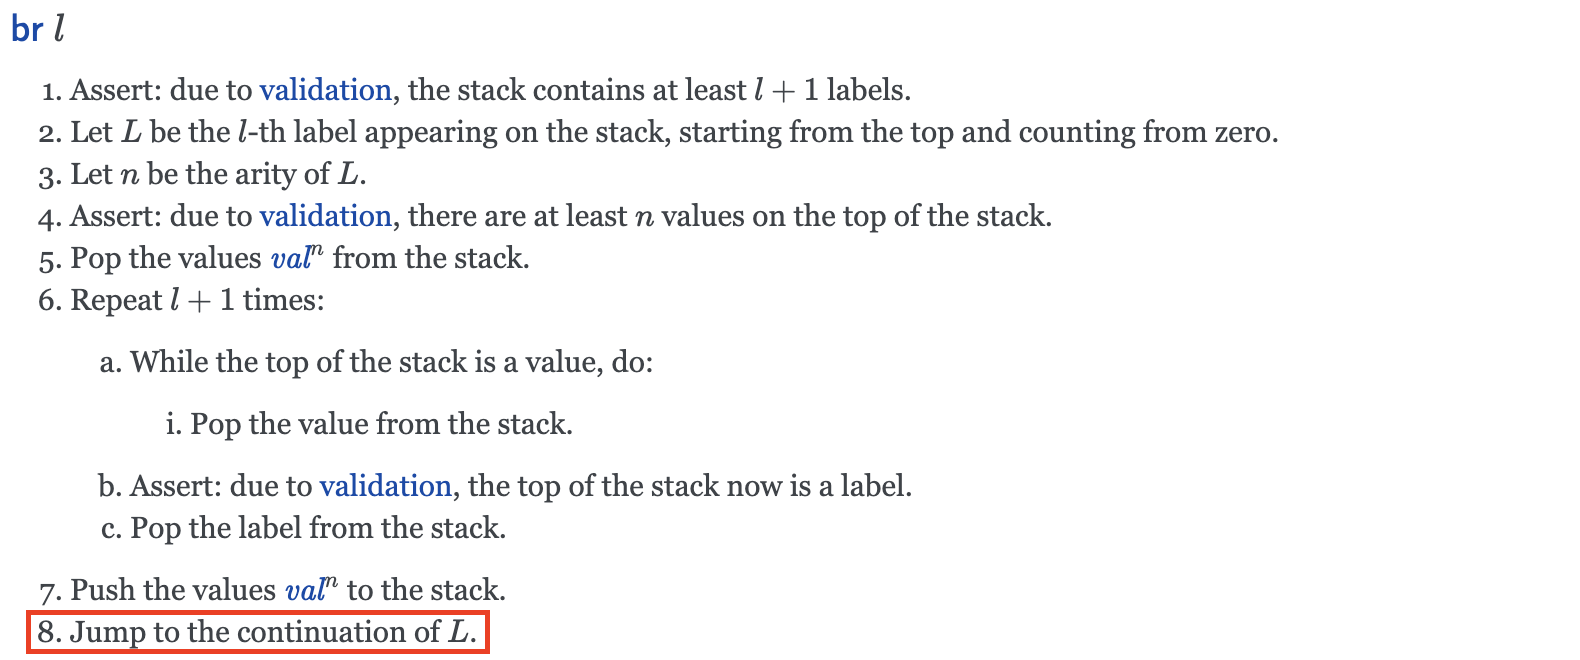
\includegraphics[width=15cm]{fig/br}}
    \caption[Enter the caption title here]{\texttt{br} instruction} \label{fig:br}
\end{figure}


% exiting label in official prose
There is also a special form of a behavior related to the block: an
\textit{exiting label}.
\cref{fig:exiting-label} is the \officialp{} of the \textit{exiting label}.
It is special because this behavior is performed without an explicit
WebAssembly instruction.
Rather, the behavior is performed when \textbf{the end of a block is reached}
without control instructions or runtime error.
The behavior is that the label is popped from the stack, and the pc changes to
the point after the end of the block.

\begin{figure}[h!]
    \centerline{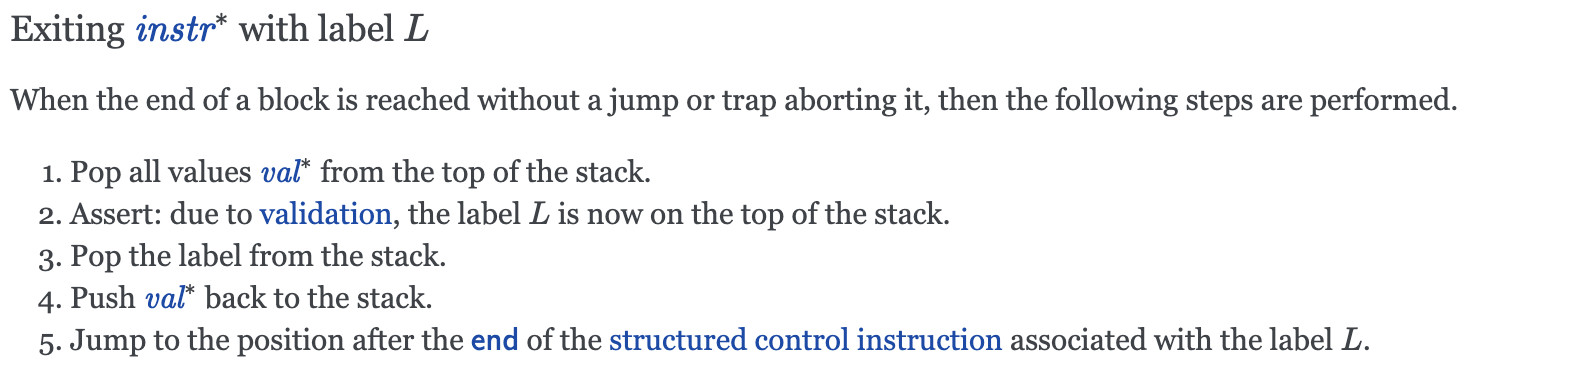
\includegraphics[width=15cm]{fig/exiting}}
    \caption[Enter the caption title here]{exiting label} \label{fig:exiting-label}
\end{figure}


% an example of exiting label in official prose
\begin{example}
\label{ex:exit}
\begin{verbatim}
  // exiting label
  (loop (result i32) (i32.const 42) end) (f64.const 3.14)
\end{verbatim}
\end{example}

\cref{ex:exit} is a WebAssembly code example that has \texttt{loop} whose block is
only \texttt{i32.const}, and \texttt{f32.const}
When the \texttt{loop} instruction is executed, it enters the block with a label.
After \texttt{i32.const} is executed, the end of the block is reached.
As a result, exiting label occurs so that the label is popped from the stack,
pc changes to the point after the end of block: \texttt{f64.const}.
As a result, after executing the code, the value 42 and 3.14 pushed to the
stack.


% control flow structure with function call in official prose
Similar to the control flow using the block and the label, there is a function
call with a frame.
\cref{fig:invoke} is the \officialp{} of the function invocation which takes
place by a \texttt{call} instruction.
A frame is pushed to the stack and enters the block of the function body with a
label.
There is also a special behavior named returning from a function.
\cref{fig:returning} is the \officialp{} of the returning from a function.
When end of function is reached without without control instructions or runtime
error, The frame is popped from the stack, and the pc points to the next
instruction of the caller instruction.

\begin{figure}[h!]
    \centerline{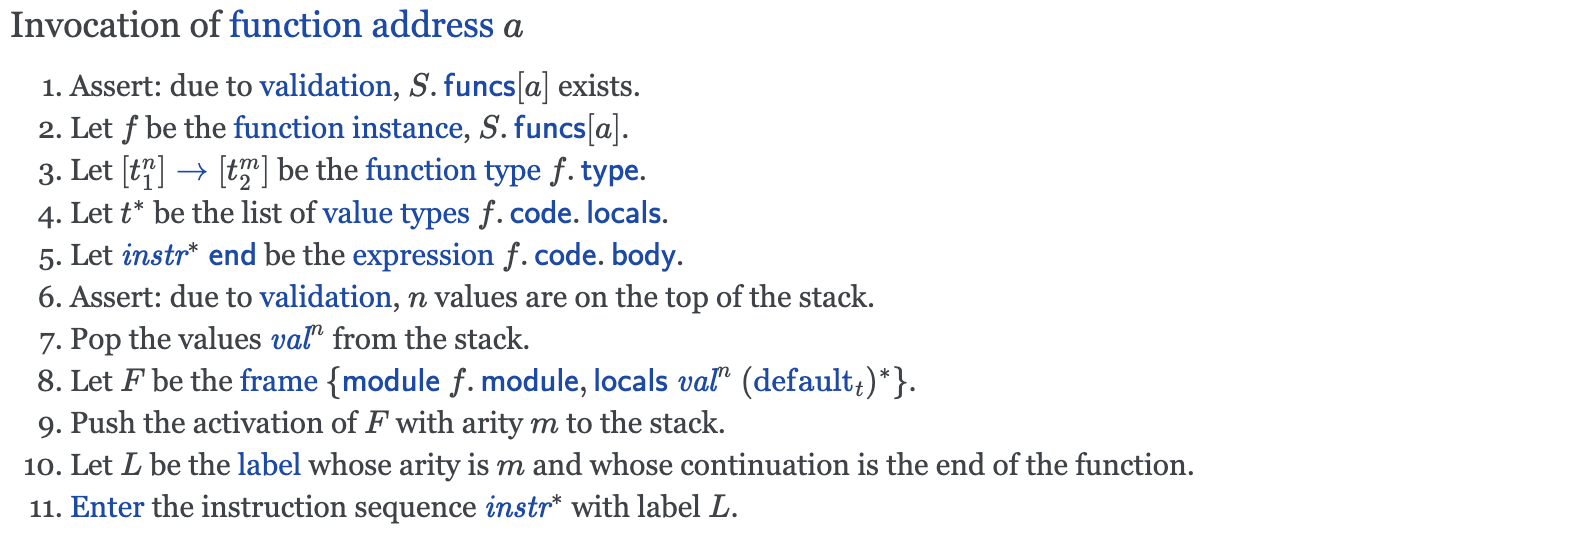
\includegraphics[width=15cm]{fig/invoke}}
    \caption[Enter the caption title here]{function invocation} \label{fig:invoke}
    \centerline{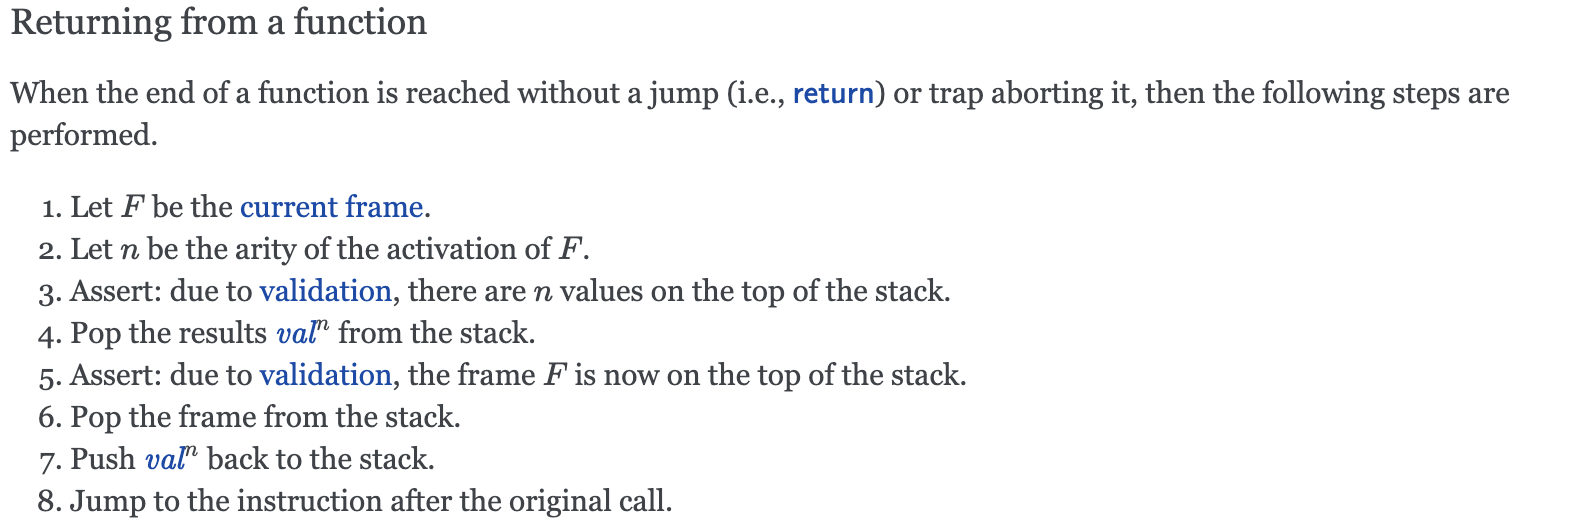
\includegraphics[width=15cm]{fig/returning}}
    \caption[Enter the caption title here]{returning from a function} \label{fig:returning}
\end{figure}

